\documentclass{beamer}
\usepackage[utf8]{inputenc}
\usepackage{pdfpages}
\usepackage{graphicx}
\usepackage{listings}
\usepackage{color}

\definecolor{mygreen}{rgb}{0,0.6,0}
\definecolor{mygray}{rgb}{0.5,0.5,0.5}
\definecolor{mymauve}{rgb}{0.58,0,0.82}

\lstset{ %
  backgroundcolor=\color{white},   % choose the background color
  basicstyle=\footnotesize,        % size of fonts used for the code
  breaklines=true,                 % automatic line breaking only at whitespace
  captionpos=b,                    % sets the caption-position to bottom
  commentstyle=\color{mygreen},    % comment style
  escapeinside={\%*}{*)},          % if you want to add LaTeX within your code
  keywordstyle=\color{blue},       % keyword style
  stringstyle=\color{mymauve},     % string literal style
  language=Java,
  basicstyle=\ttfamily
}

\lstset{literate=%
{Ö}{{\"O}}1
{Ä}{{\"A}}1
{Ü}{{\"U}}1
{ß}{{\ss}}2
{ü}{{\"u}}1
{ä}{{\"a}}1
{ö}{{\"o}}1
}

\usetheme{Berkeley}

\title{PK0}
\subtitle{Zusatzkurs für Programmieranfänger im WS 16/17}
\author{Marvin Gülzow}
\institute{Universität Konstanz}
\date{2016-11-02}

\begin{document}
\frame{\maketitle}

\begin{frame}
\frametitle{Inhalt}
\tableofcontents
\end{frame}

\section{Kontext}
\subsection{Transistoren}
\begin{frame}{\subsecname}
  \centering
  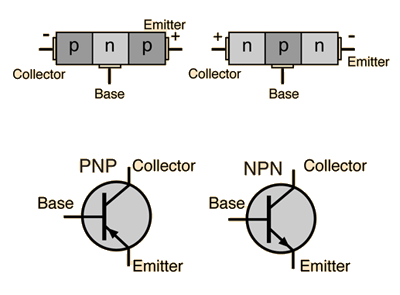
\includegraphics[width=\textwidth]{img/01_transistor.png}  
\end{frame}

\begin{frame}{\subsecname}
  \centering
  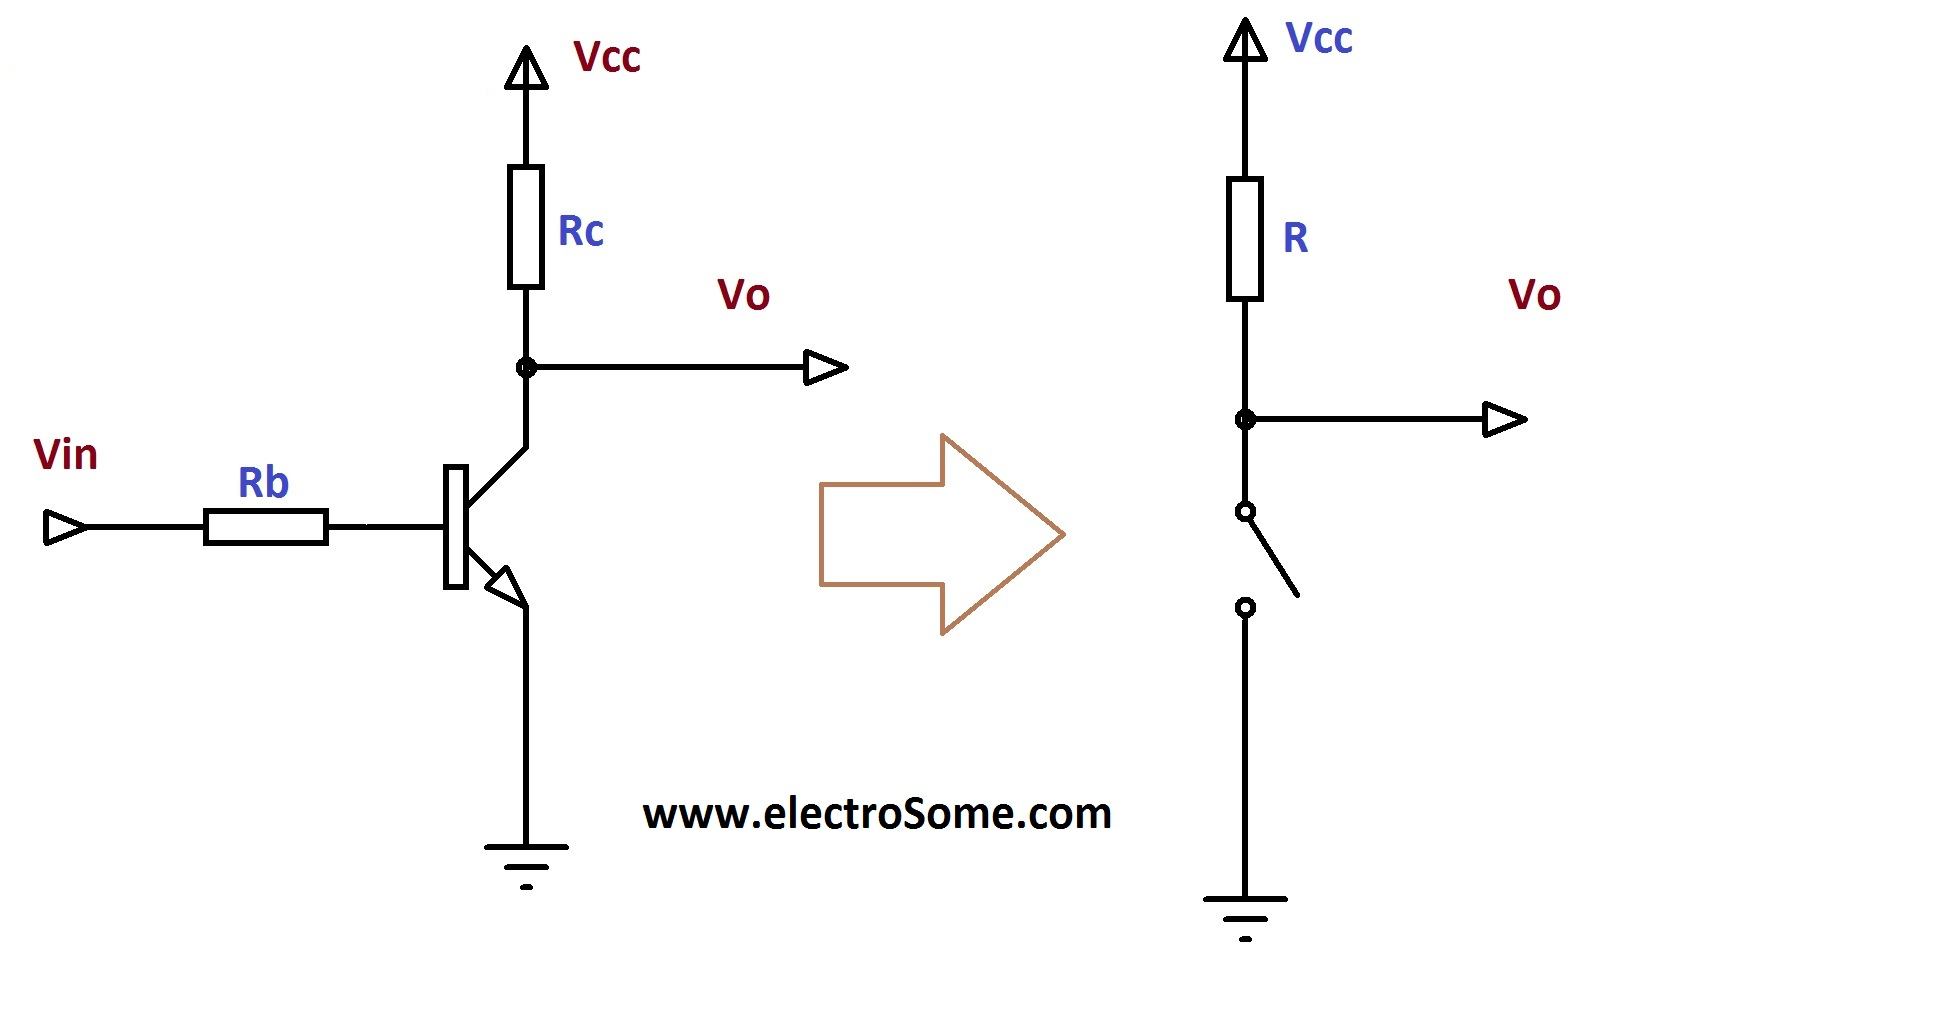
\includegraphics[width=\textwidth]{img/02_switch.jpg}  
\end{frame}

\begin{frame}{\subsecname}
  \centering
  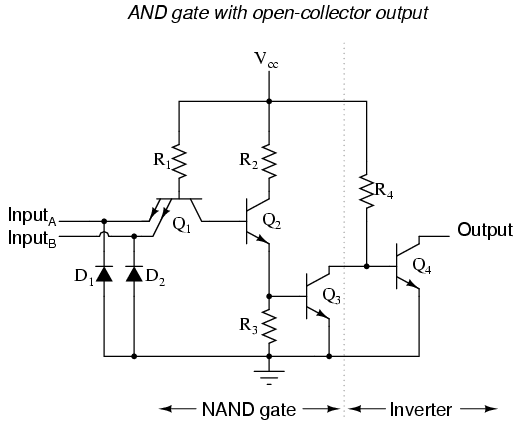
\includegraphics[width=\textwidth]{img/andgate.png}  
\end{frame}

\begin{frame}{\subsecname}
  \centering
  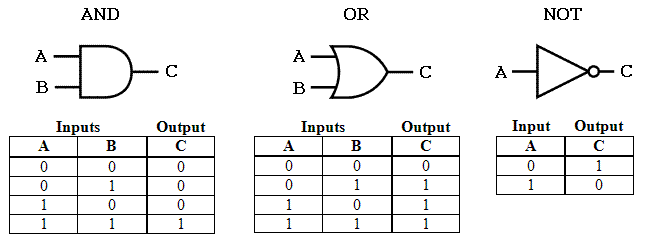
\includegraphics[width=\textwidth]{img/truthtables.png}  
\end{frame}

\begin{frame}{\subsecname}
  \centering
  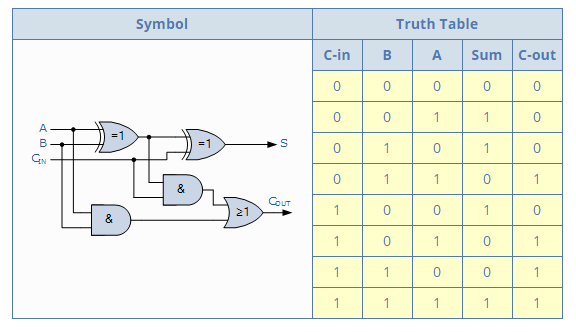
\includegraphics[width=\textwidth]{img/03_adder.png}  
\end{frame}

\subsection{Prozessor}
\begin{frame}{\subsecname}
  \centering
  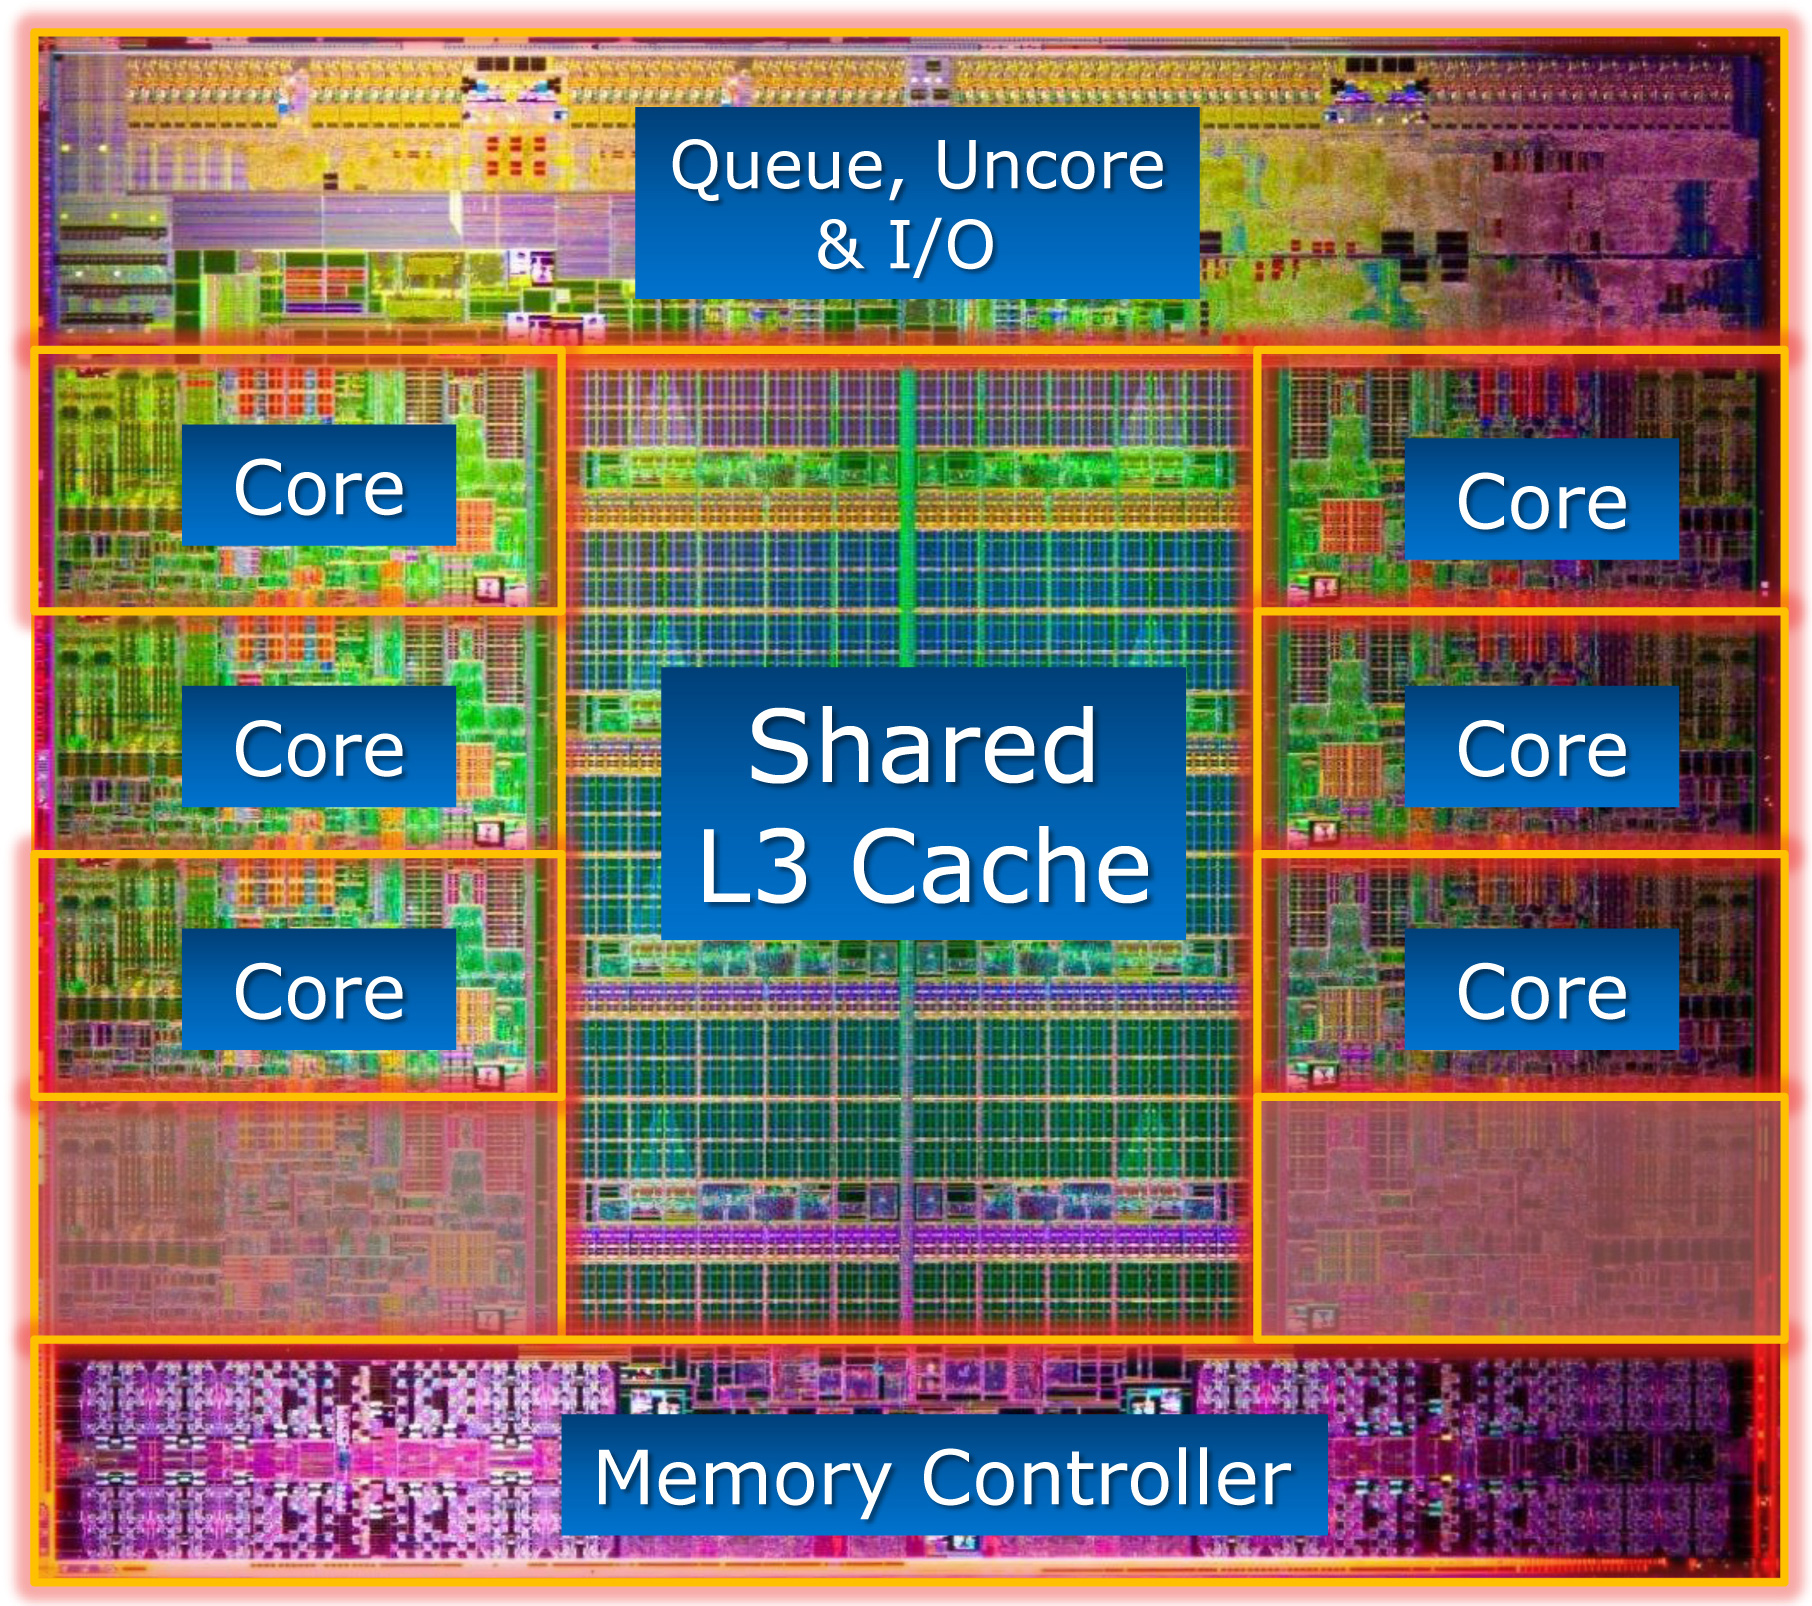
\includegraphics[width=\textwidth]{img/05_cpu.jpg}  
\end{frame}

\begin{frame}{\subsecname}
  \centering
  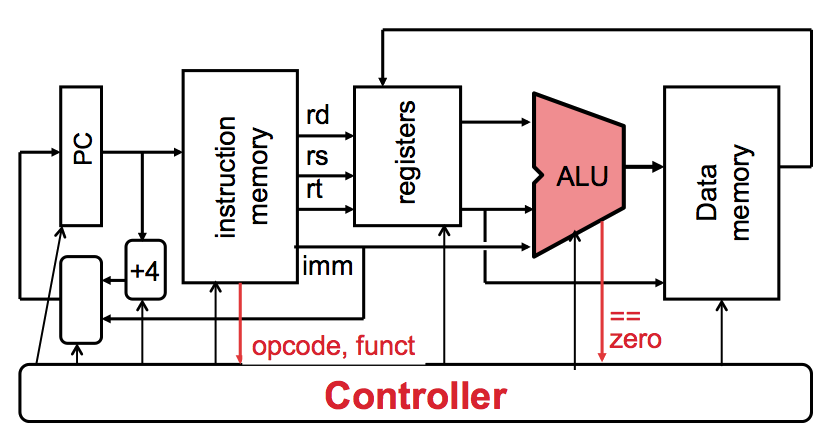
\includegraphics[width=\textwidth]{img/04_alu.png}  
\end{frame}

\begin{frame}{\subsecname}
  \centering
  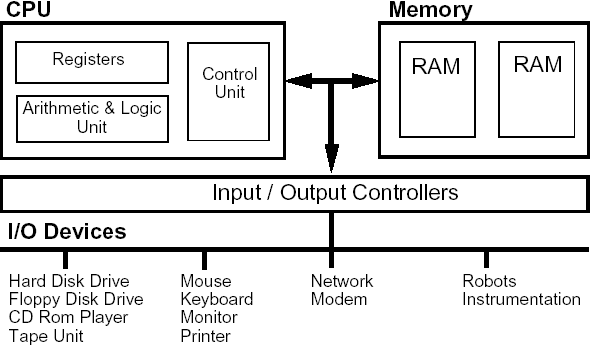
\includegraphics[width=\textwidth]{img/06_overall.png}  
\end{frame}

\subsection{Programme}
\begin{frame}[fragile]{\subsecname}
  \begin{lstlisting}
_start:
	mov cx, 10
	mov esi, 0
loop:
	inc esi
	dec cx
	jnz loop
  \end{lstlisting}

  $\Rightarrow$ b90a 0066 be00 0000 0066 4649 75fb
\end{frame}

\begin{frame}[fragile]{\subsecname}
  \begin{lstlisting}
int c = 10;
int e = 0;

while(c > 0) {
    ++e; // e = e + 1
    --c;
}
  \end{lstlisting}
  
  \begin{lstlisting}
_start:
	mov cx, 10
	mov esi, 0
loop:
	inc esi
	dec cx
	jnz loop
  \end{lstlisting}
\end{frame}

\begin{frame}{\subsecname}
  \centering
  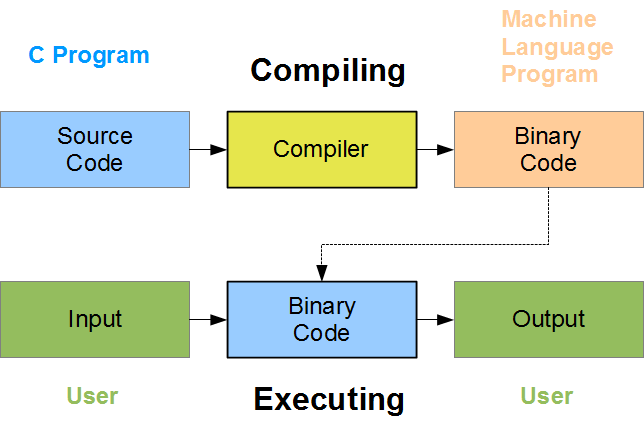
\includegraphics[width=\textwidth]{img/compiler.png}  
\end{frame}

\subsection{JVM}
\begin{frame}{\subsecname}
  \centering
  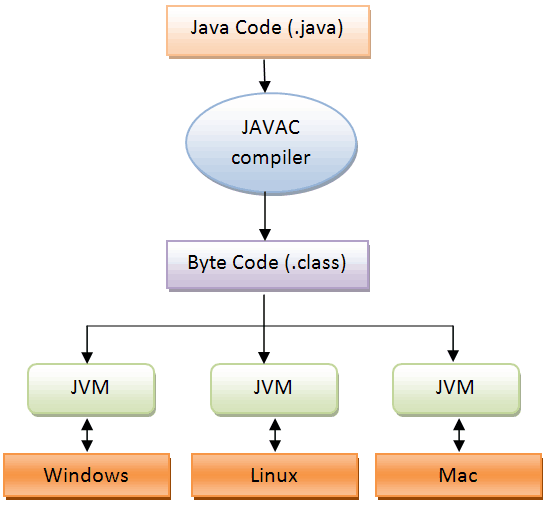
\includegraphics[height=\textheight]{img/java-program-execution.png}  
\end{frame}

\begin{frame}[fragile]{\subsecname}
  \begin{lstlisting}
int i = 0;
i += 1;
i = i * 2
    
iconst_0      // 03
istore_0      // 3b
iinc 0, 1     // 84 00 01
iload_0       // 1a
iconst_2      // 05
imul          // 68
istore_0      // 3b
goto -7       // a7 ff f9
  \end{lstlisting}
  $\Rightarrow$ 03 3b 84 00 01 1a 05 68 3b a7 ff f9
\end{frame}

\begin{frame}{\subsecname}
  \begin{enumerate}
  \item Javacode schreiben
  \item Bytecode
  \item JVM
  \item Bytes im RAM
  \item Elektronen in der CPU
  \item Quantenmechanik
  \end{enumerate}
\end{frame}

\begin{frame}{\subsecname}
  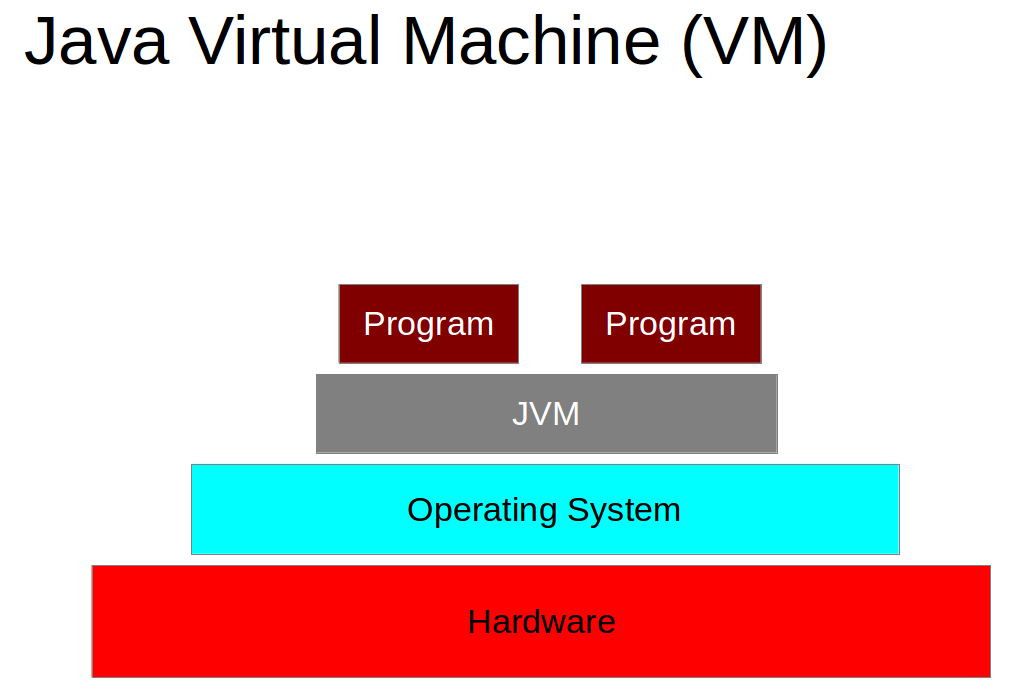
\includegraphics[width=\textwidth]{img/osstack.png}  
\end{frame}

\section{Statements und Bedingungen}
\subsection{Statements}
\begin{frame}[fragile]{\subsecname}
  \begin{lstlisting}
int i = 0;
int x = 1;

i = 1;     // 1
i = 2;     // 2
i = i + 1; // 3
i = i + x; // 4
i += 1;    // 5
i += x;    // 6
++i;       // 7
i++;       // 8
  \end{lstlisting}
\end{frame}

\begin{frame}[fragile]{\subsecname}
  \begin{lstlisting}
int i = 0;
int x = 1;

i = i + 2; // 2
i = i - 1; // 1
i = i * 2; // 2
i = i / 2; // 1
i = i + 2; // 3 :)
i = i / 2; // 1 WTF?
  \end{lstlisting}
\end{frame}

\begin{frame}[fragile]{\subsecname}
  \begin{lstlisting}
int i = 0;
int x = 1;

i = i + x;   i += x; // Addition
i = i - x;   i -= x; // Subtraktion
i = i * x;   i *= x; // Multiplikation
i = i / x;   i /= x; // Division
i = i % x;   i %= x; // Modulo
  \end{lstlisting}
\end{frame}

\begin{frame}[fragile]{\subsecname}
  \begin{lstlisting}
int i = 0;

++i;
i += 1;

i++;
int tmp = i;
i += 1;
return tmp;
  \end{lstlisting}
\end{frame}

\begin{frame}[fragile]{\subsecname}
  \begin{lstlisting}
int i = 0;
int x = 0;

x = ++i;   // x == 1 == i
x = i++;   // x == 1; i == 2; 
  \end{lstlisting}
  $\Rightarrow$ Benutzt ++i.
\end{frame}

\subsection{Evaluation}
\begin{frame}[fragile]{\subsecname}
  \begin{lstlisting}
int a = 1 + 2 * 3;   // 7
int b = (1 + 2) * 3; // 9
  \end{lstlisting}
  \begin{itemize}
  \item Alles Klammern
  \item Klammern sind billig
  \item Keiner kann sich alle Operatoren merken
  \end{itemize}
\end{frame}

\begin{frame}[fragile]{\subsecname}
  \begin{lstlisting}
int i = 0;
int x = 1;

i == x;     // false
i != x;     // true
i < x;      // true
i > x;      // false
(i+1) <= x; // true;
i >= x;     // false;

boolean comparison = i == x;

comparison += 1; // Nein.
  \end{lstlisting}
\end{frame}

\subsection{Bedingungen}
\begin{frame}[fragile]{\subsecname}
  \begin{lstlisting}
int i = 0;
int x = 1;

if (i == x) {
  System.out.println("Equal.");
}

if (i != x) {
  System.out.println("Not equal.");
}
  \end{lstlisting}
\end{frame}

\begin{frame}[fragile]{\subsecname}
  \begin{lstlisting}
int i = 0;
int x = 1;

if (i == x) {
  System.out.println("Equal.");
} else  {
  // Fall (i != x)
  System.out.println("Not equal.");
}
  \end{lstlisting}
\end{frame}

\begin{frame}[fragile]{\subsecname}
  \begin{lstlisting}
int i = 0;
int x = 1;

if (i == x) {
  System.out.println("Equal.");
} else if (i != x)  {
  System.out.println("Not equal.");
} else {
  System.out.println("CPU is broken.");
}
  \end{lstlisting}
\end{frame}

\begin{frame}[fragile]{\subsecname}
  \begin{lstlisting}
int i = 0;
int x = 1;

boolean comparison = (i == x);

if (comparison == true) {
  System.out.println("Equal.");
} else if (compariosn == false)  {
  System.out.println("Not equal.");
} else {
  System.out.println("CPU is broken.");
}
  \end{lstlisting}
\end{frame}

\begin{frame}[fragile]{\subsecname}
  \begin{lstlisting}
int i = 0;
int x = 1;

boolean comparison = (i == x);

if (comparison) {
  System.out.println("Equal.");
} else if (!comparison)  {
  System.out.println("Not equal.");
} else {
  System.out.println("CPU is broken.");
}
  \end{lstlisting}
\end{frame}

\begin{frame}[fragile]{\subsecname}
  \begin{lstlisting}
mov esa, 0
mov esb, 1

cmp i, x
je equal
jne notequal

print "CPU broken"
ret
equal:
print "Equal"
ret
notequal:
print "Notequal"
ret

  \end{lstlisting}
\end{frame}

\section{Fazit}
\begin{frame}{\secname}
  \begin{itemize}
  \item Alles ist kompliziert
  \item Alles basiert auf einem riesigen Technikstack
  \item Der Übergang von Ideen des Programmierers zu Elektronen in Silizium ist über Layer gelöst
  \item Die Technik ganz unten formt die Sprachen ganz oben
    \begin{itemize}
    \item Ultraschnelles Addieren
    \item Alles ist zahlenbasiert
    \item Daten/Programm-Dualität
    \end{itemize}
  \item Wer den ganzen Stack im Hinterkopfe hat versteht besser was er/sie/es tut
  \item Nächstes mal: Mehr praktisches :)
  \end{itemize}
\end{frame}

\end{document}
